% ---------------------------------------------------------------
% Section: Particle Tracking Pipeline
% ---------------------------------------------------------------

\section[Particle Tracking]{Particle Tracking Pipeline}

\begin{frame}{From Detection to Tracking}
\begin{columns}
\begin{column}{0.55\textwidth}
\textbf{Detection output (per frame):}
\begin{itemize}\small
    \item Anonymous $(x_i, y_i, \varphi_i)$ — no persistent identity
    \item Missed frames break the time series
    \item Duplicate detections per particle possible
\end{itemize}
\smallskip
\textbf{What tracking adds:}
\begin{itemize}\small
    \item Persistent \texttt{track\_id} across all frames
    \item Continuous trajectories $(x(t),\, y(t),\, \varphi(t))$
    \item Filled gaps flagged as \texttt{is\_interpolated}
    \item Foundation for physics analysis
\end{itemize}
\end{column}
\begin{column}{0.45\textwidth}
\textbf{Three-stage pipeline}\\
(\texttt{src/track\_particles.py}):
\begin{enumerate}\small
    \item \textbf{Within-frame NMS}\\
          Remove duplicate detections
    \item \textbf{Hungarian linking}\\
          Optimal cross-frame assignment
    \item \textbf{Gap interpolation}\\
          Recover short missed segments
\end{enumerate}
\end{column}
\end{columns}
\end{frame}

\begin{frame}{Stage 1 — Within-Frame NMS}
\begin{columns}
\begin{column}{0.55\textwidth}
\textbf{Problem:} LodeSTAR produces multiple nearby detections for one physical particle (cluster of high-confidence pixels converging on one centre).

\smallskip
\textbf{Non-Maximum Suppression:}
\begin{enumerate}\small
    \item Sort detections by NCC score (highest first)
    \item Suppress all neighbours within $r_{\min} = 20$ px
    \item \texttt{scipy.spatial.cKDTree} for efficient queries
\end{enumerate}
\smallskip
\textbf{Result:} one detection per particle per frame.
\end{column}
\begin{column}{0.45\textwidth}
\begin{center}
\small\textbf{Config parameter:}\\[0.2cm]
\begin{tabular}{|l|c|}
\hline
\texttt{min\_det\_distance} & 20 px \\
\hline
\end{tabular}
\end{center}
\smallskip
\begin{mynote}[Why score-based?]
\small Keeping the highest-NCC detection (not just the first found) gives the most reliable centre for the subsequent linking step.
\end{mynote}
\end{column}
\end{columns}
\end{frame}

\begin{frame}{Stage 2 — Hungarian Cross-Frame Linking}
\begin{columns}
\begin{column}{0.58\textwidth}
\textbf{Hungarian algorithm:}
\begin{itemize}\small
    \item Cost matrix: Euclidean distance, active tracks $\times$ new detections
    \item \texttt{scipy.optimize.linear\_sum\_assignment} → globally optimal ($O(n^3)$)
    \item Pairs beyond \texttt{max\_link\_distance} rejected
\end{itemize}
\smallskip
\textbf{Track state machine:}\\[0.2cm]
\small\begin{tabular}{|l|l|}
\hline
\textbf{Event} & \textbf{Action} \\
\hline
Detection matched  & Update track position \\
\hline
Detection unmatched & Start new \texttt{track\_id} \\
\hline
Track unmatched     & gap $\leftarrow$ gap+1 \\
\hline
gap $>$ max\_gap    & Terminate track \\
\hline
\end{tabular}
\end{column}
\begin{column}{0.42\textwidth}
\begin{center}
\small\textbf{Parameters:}\\[0.2cm]
\begin{tabular}{|l|c|}
\hline
\texttt{max\_link\_dist} & 30 px \\
\hline
\texttt{min\_track\_len} & 5 fr \\
\hline
\texttt{max\_gap\_frames} & 10 fr \\
\hline
\end{tabular}
\end{center}
\smallskip
\begin{mynote}
\small Crossing particles create a short gap in each track — recovered in Stage 3.
\end{mynote}
\end{column}
\end{columns}
\end{frame}

\begin{frame}{Stage 3 — Gap Interpolation}
\begin{columns}
\begin{column}{0.55\textwidth}
\textbf{Rules for gaps $\leq$ 10 frames:}
\begin{itemize}\small
    \item $x$, $y$: linear interpolation
    \item $\varphi$: circular — $\Delta\varphi = [(\varphi_b - \varphi_a + \pi) \bmod 2\pi] - \pi$
    \item Filled rows flagged \texttt{is\_interpolated = True}
\end{itemize}
\smallskip
\small\begin{tabular}{|l|r|}
\hline
\textbf{Quantity} & \textbf{Value} \\
\hline
Total tracks      & 1{,}173 \\
\hline
Total rows        & 120{,}597 \\
\hline
Interpolated (10\%) & 12{,}279 \\
\hline
Real detections   & 108{,}318 \\
\hline
\end{tabular}
\end{column}
\begin{column}{0.45\textwidth}
\begin{mynote}[Combined tracking]
\footnotesize All 11 videos merged with continuous frame numbering — eliminates jumps at video boundaries.
\end{mynote}
\smallskip
\begin{myalert}[Limitation]
\footnotesize Linear interpolation assumes constant velocity. For ABP particles this is a first-order approximation — see Future Work for physics-informed alternatives.
\end{myalert}
\end{column}
\end{columns}
\end{frame}

\begin{frame}{Track Visualisation — All Trajectories}
\centering
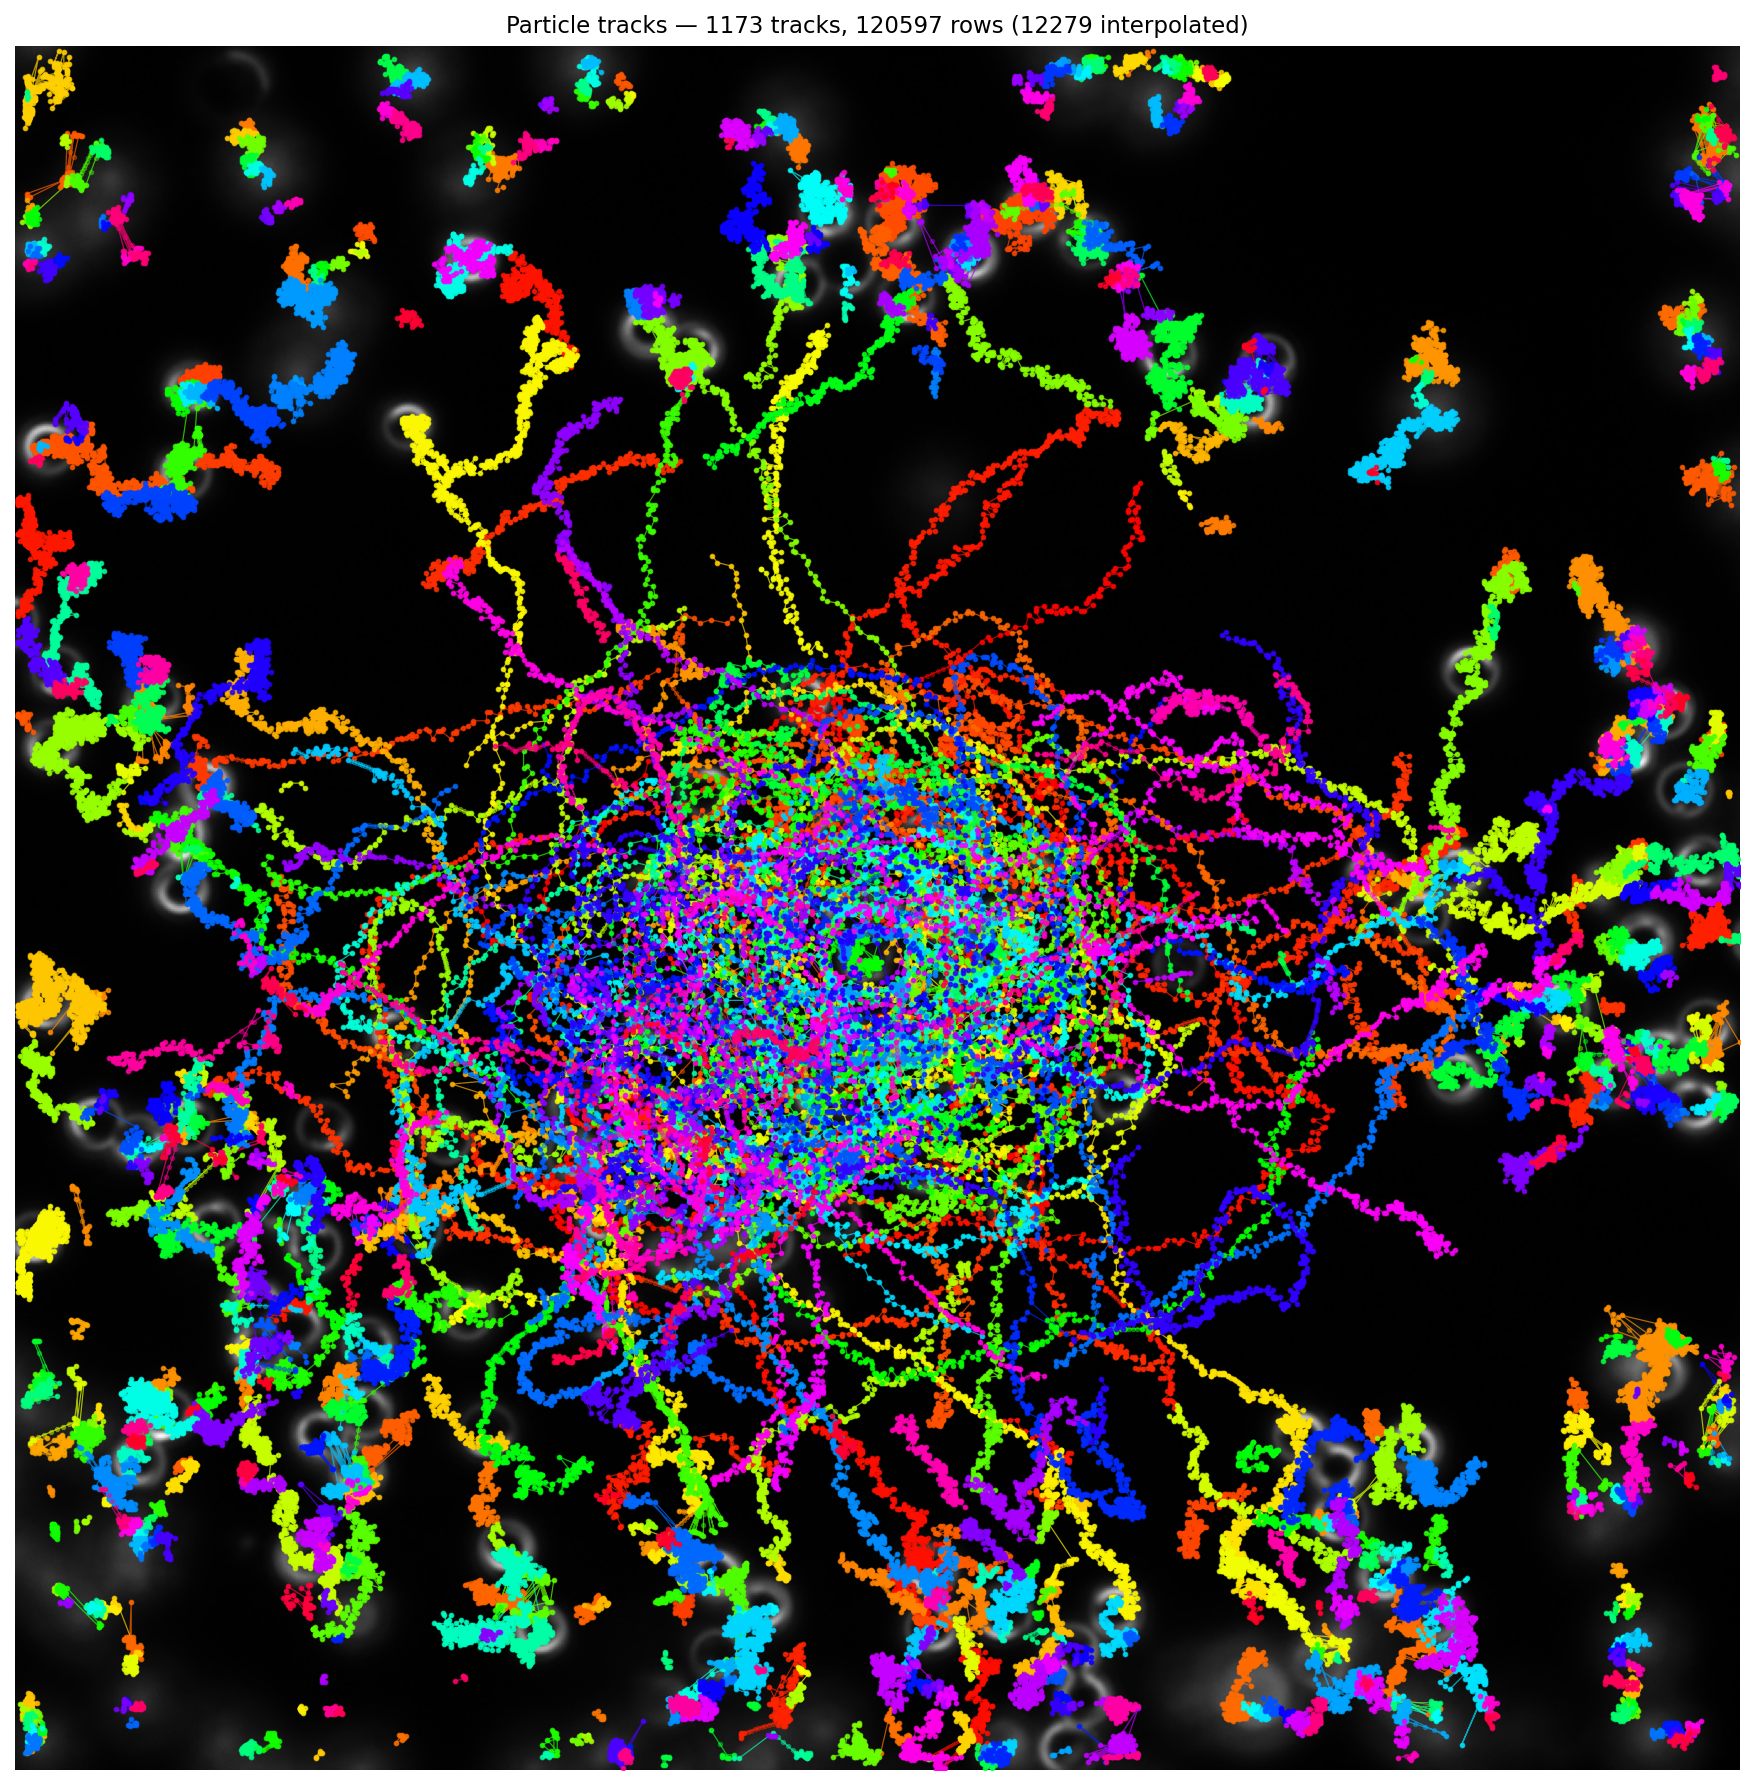
\includegraphics[width=\textwidth, height=0.76\textheight, keepaspectratio]{imglib/tracking/tracks_overview.png}\\
{\footnotesize All 1{,}173 tracks on mid-frame background. Colours: distinct particles.}
\end{frame}

\begin{frame}{Sample Trajectories — 12 Longest Tracks}
\centering
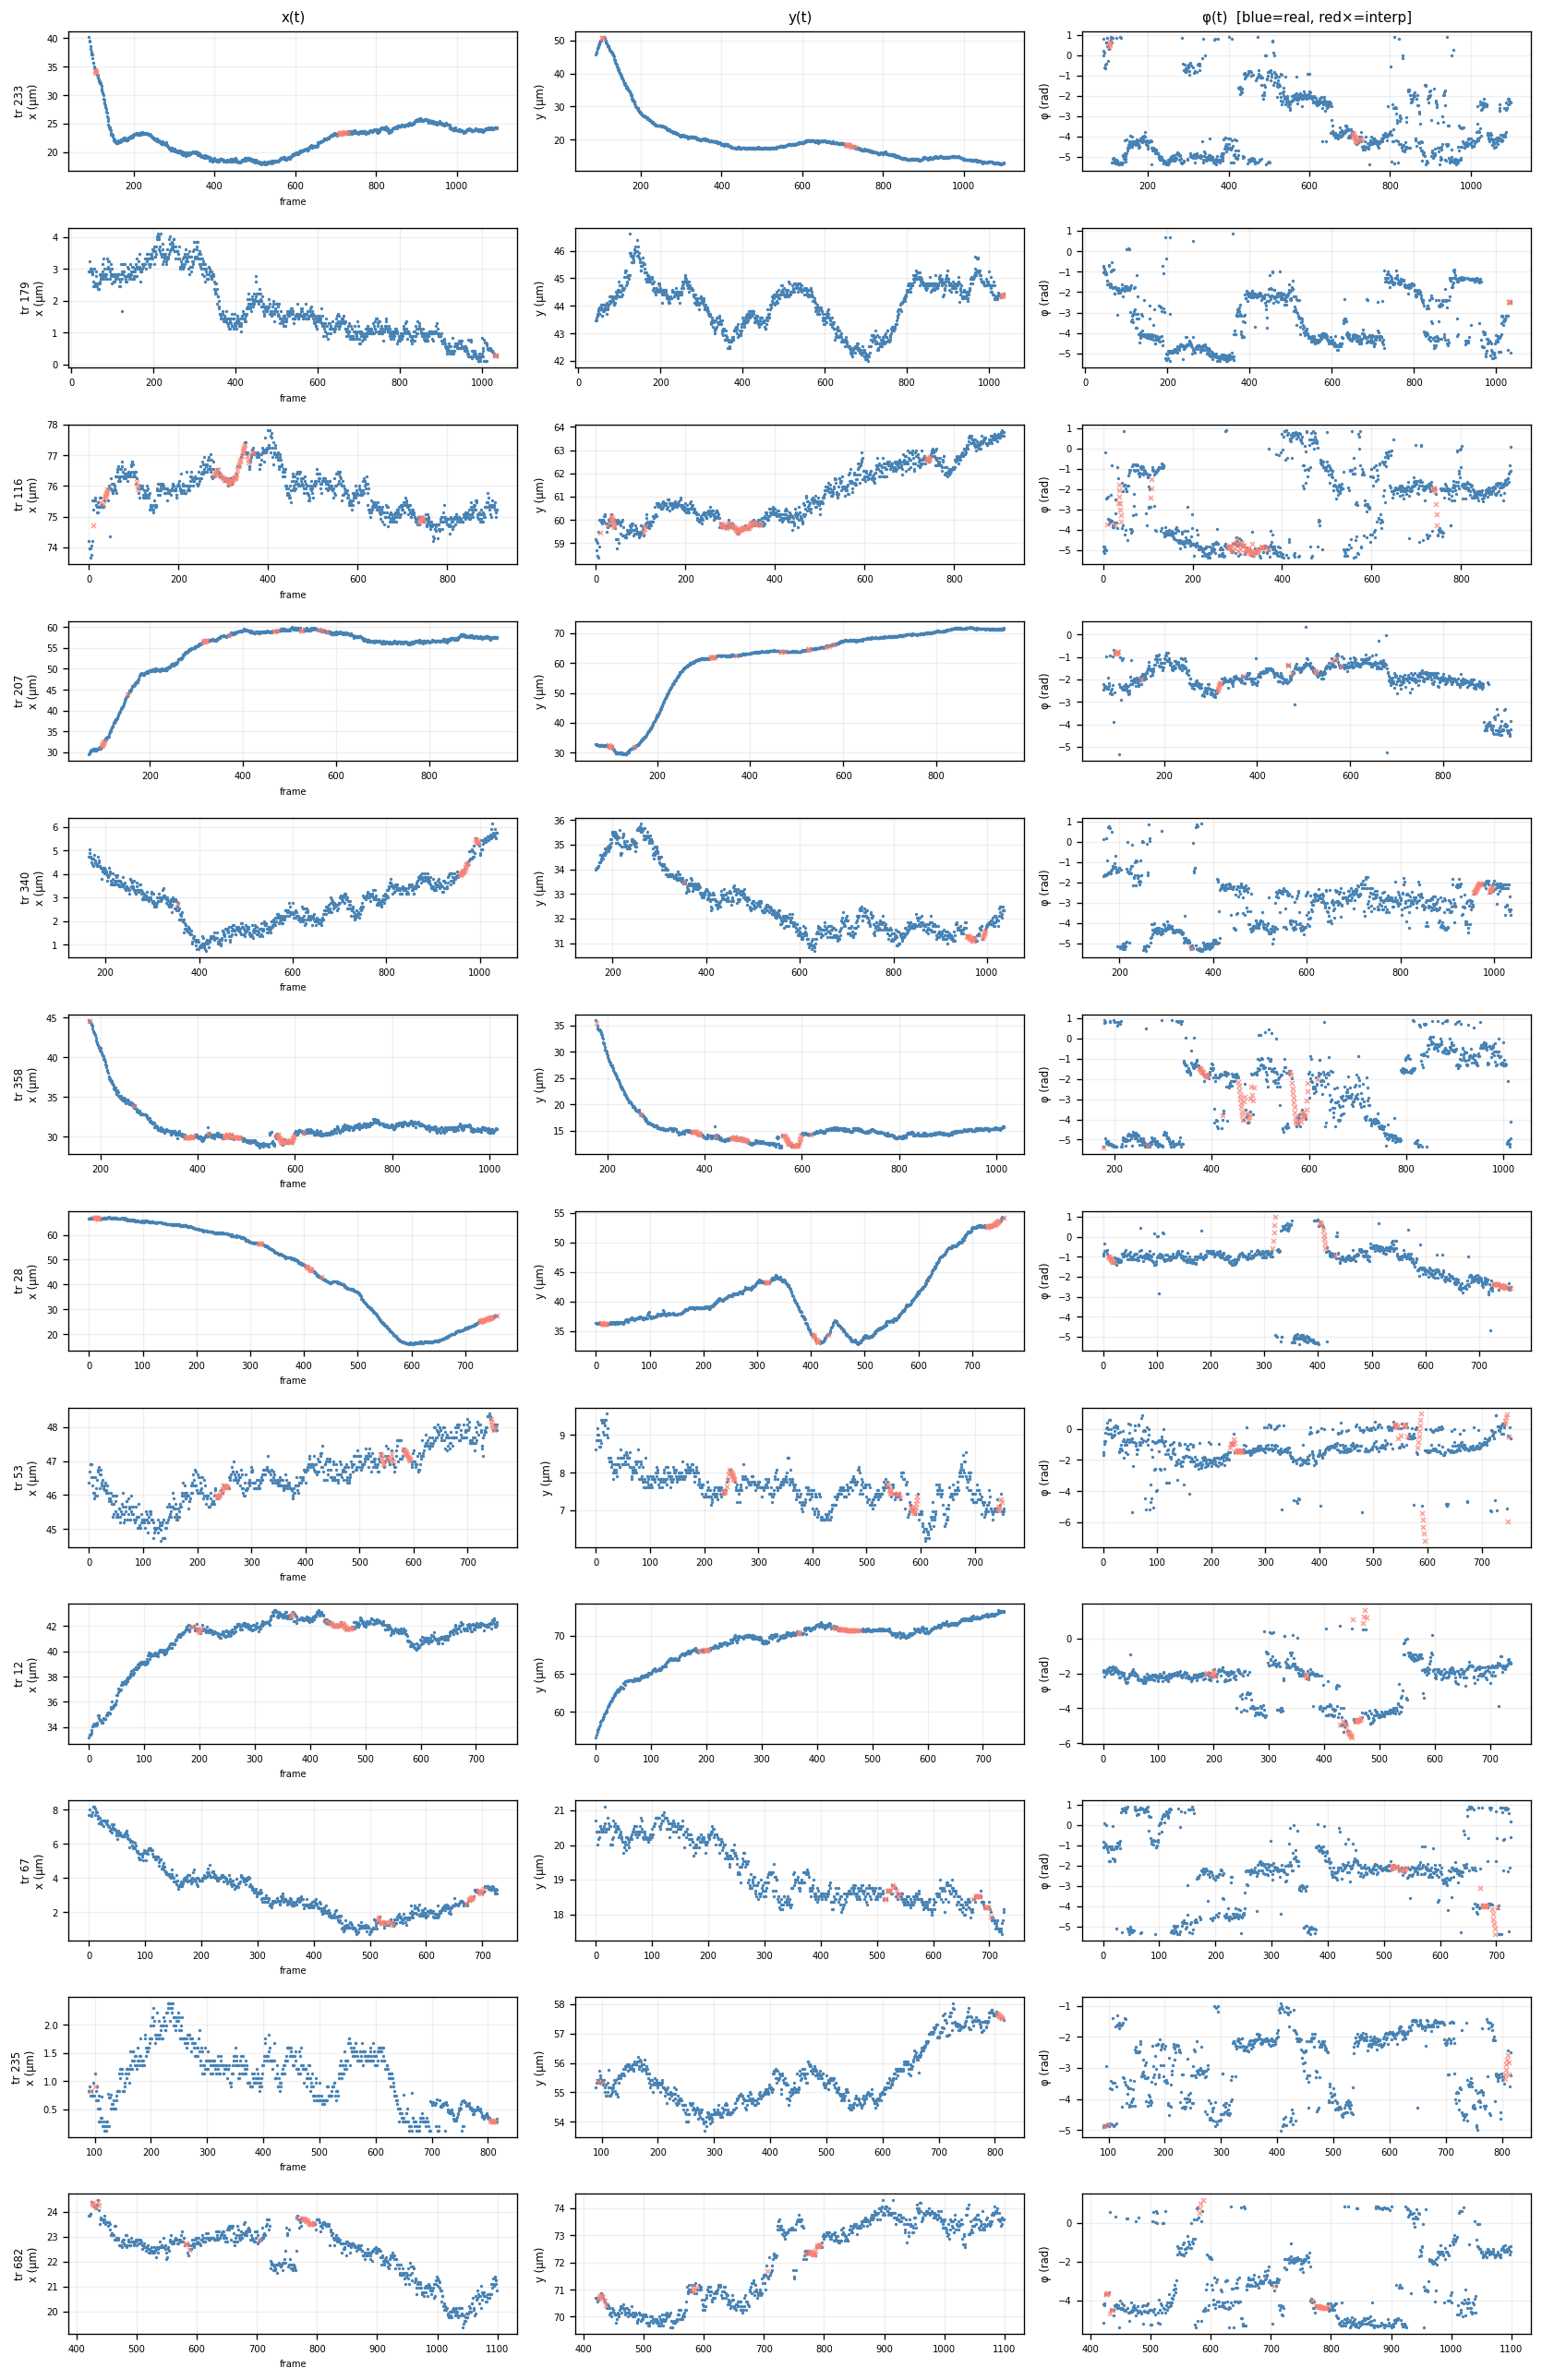
\includegraphics[width=\textwidth, height=0.76\textheight, keepaspectratio]{imglib/tracking/tracks_sample_tracks.png}\\
{\footnotesize $x(t)$, $y(t)$, $\varphi(t)$. Blue: real detections; red $\times$: interpolated.}
\end{frame}
